\entry{Semana del 01/09/2025.} 

\section{Lunes 01/09/2025} 

\subsection*{PDFs de FCD}
Siguiendo con el análisis de las mediciones obtenidas con FCD me puse a calcular las PDFs de las alturas. Para esto probé dos opciones, o calcular un histograma por píxel usando los datos temporales y después promediarlos todos, u obtener un histograma por frame y después promediar estos (este último no medio resultados muy razonables). En todos los casos está la altura normalizada por la desviación estándar y tiene media 0. 



\begin{figure}[!ht]
	\begin{minipage}[c]{0.325\textwidth}
			\begin{subfigure}{\textwidth}
					\centering
					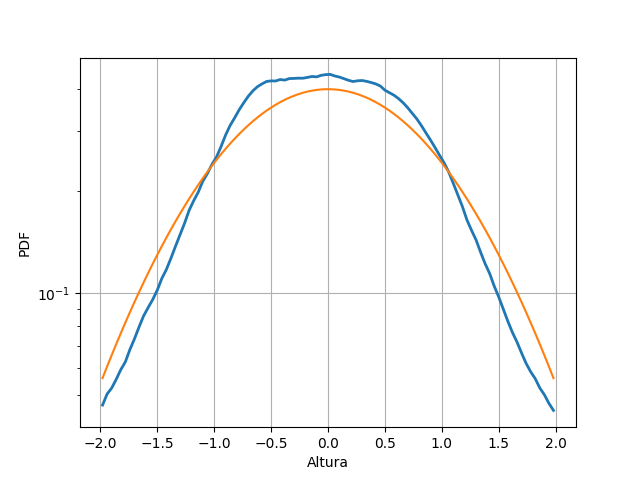
\includegraphics[width=0.98\textwidth]{Figures/01_09_2025/PDF_FCD_amp10.png}
					\captionsetup{width=0.8\textwidth}
					\subcaption{Amplitud 10 \%.}
					% \label{fig:}
				\end{subfigure}
		\end{minipage}\begin{minipage}[c]{0.3249\textwidth}
			\begin{subfigure}{\textwidth}
					\centering
					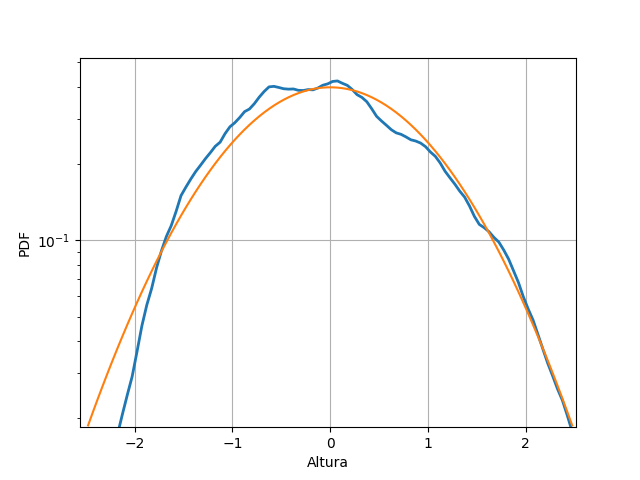
\includegraphics[width=0.98\textwidth]{Figures/01_09_2025/PDF_FCD_amp30.png}
					\captionsetup{width=0.8\textwidth}
					\subcaption{Amplitud 30 \%.}
					% \label{fig:}
				\end{subfigure}
		\end{minipage}\begin{minipage}[c]{0.3249\textwidth}
			\begin{subfigure}{\textwidth}
					\centering
					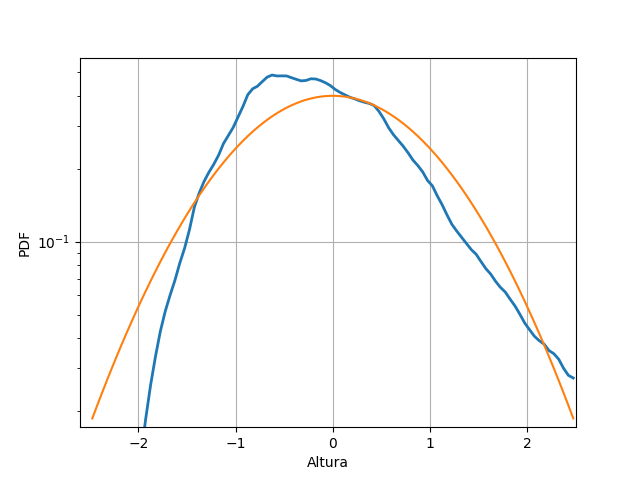
\includegraphics[width=0.98\textwidth]{Figures/01_09_2025/PDF_FCD_amp50.png}
					\captionsetup{width=0.8\textwidth}
					\subcaption{Amplitud 50 \%.}
					% \label{fig:}
				\end{subfigure} 
		\end{minipage}
	\caption{PDFs con media 0 y desviación estándar unidad para distintas amplitudes de forzado en la banda 0 - 4 Hz, a partir de un promedio entre píxeles de la región central de 300 x 300 px$^2$ a partir de la reconstrucción con FCD de la superficie libre en la cuba chica. }
	\label{fig:PDFS_FCD}
\end{figure}

Podemos notar una progresión a medida que aumentamos la intensidad del forzado, donde se va volviendo más asimétrica cada vez la PDF, pero para la amplitud más baja que esperaríamos sea lo más parecido a una Gaussiana resulta ser más achatada, no me queda muy claro porqué. 

\subsection*{PDFs de las Fases.} 
Siguiendo con los análisis de las mediciones de la cuba chica con el sensor capacitivo quisimos ver la evolución de las fases hacia la aleatoriedad en el forzado de mayor intensidad. Probé varias ventanas y utilizando o no unwrapping después de hacer la FFT. 

\begin{figure}[!ht]
	\begin{minipage}[c]{0.5\textwidth}
				\begin{subfigure}{\textwidth}
							\centering
							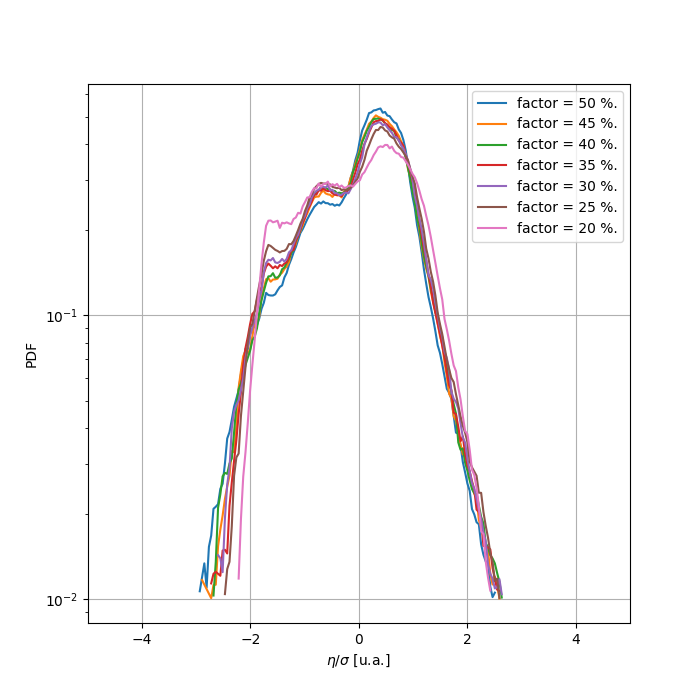
\includegraphics[width=0.6709809\textwidth]{Figures/01_09_2025/Fases_sin_unwrap_ventana_3s.png}
							\captionsetup{width=0.8\textwidth}
							\subcaption{Ventana de 3 s.}
							% \label{fig:}
						\end{subfigure}
			\end{minipage}\begin{minipage}[c]{0.49\textwidth}
				\begin{subfigure}{\textwidth}
							\centering
							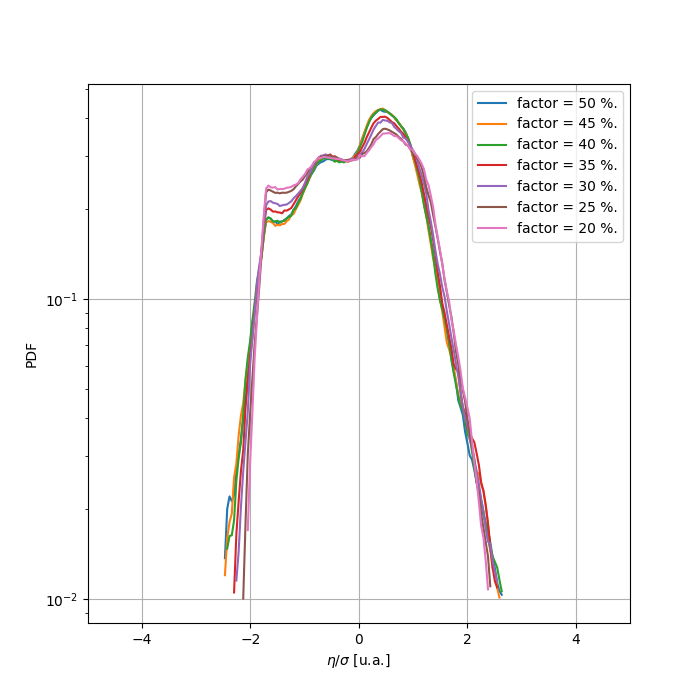
\includegraphics[width=0.6709809\textwidth]{Figures/01_09_2025/Fases_sin_unwrap_ventana_10s.png}
							\captionsetup{width=0.8\textwidth}
							\subcaption{Ventana de 10 s.}
							% \label{fig:}
						\end{subfigure}
			\end{minipage}
	\caption{PDFs de las fases en ventanas temporales de los datos en la banda de 0 - 4 Hz para las distintas amplitudes, sin realizar unwrapping luego de calcularla.}
	\label{fig:pdfs_fases_sin_unwrapping}
\end{figure} 

Sin el unwrapping queda algo asimétrico con tres picos que no me queda claro qué son.  

\begin{figure}[!ht]
	\begin{minipage}[c]{0.5\textwidth}
				\begin{subfigure}{\textwidth}
							\centering
							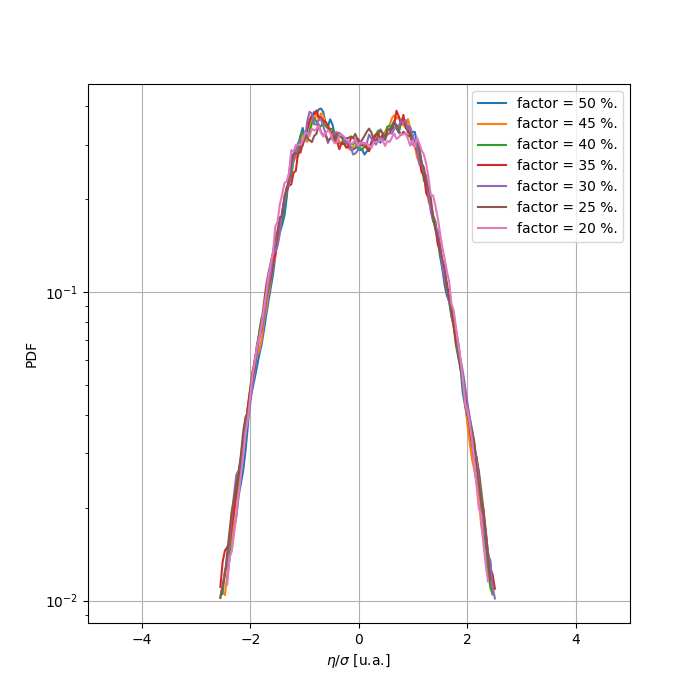
\includegraphics[width=0.6709809\textwidth]{Figures/01_09_2025/Fases_con_unwrap_ventana_3s.png}
							\captionsetup{width=0.8\textwidth}
							\subcaption{Ventana de 3 s.}
							% \label{fig:}
						\end{subfigure}
			\end{minipage}\begin{minipage}[c]{0.49\textwidth}
				\begin{subfigure}{\textwidth}
							\centering
							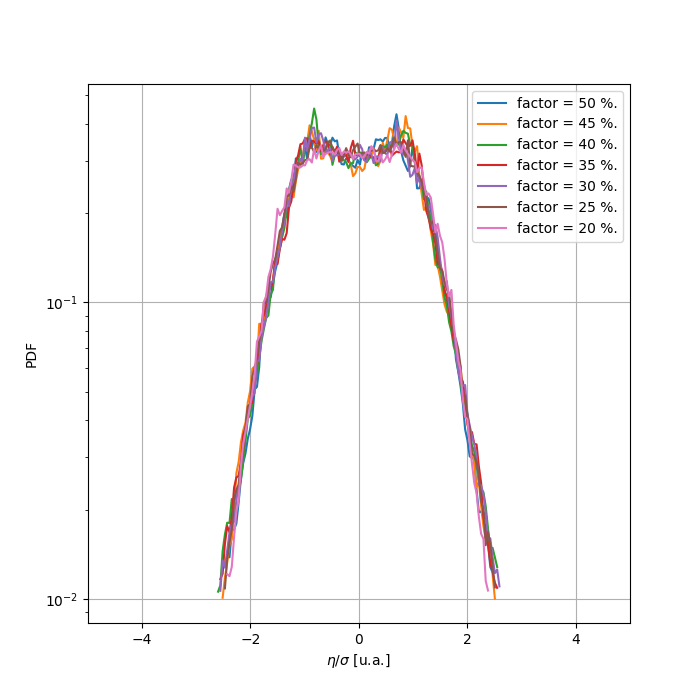
\includegraphics[width=0.6709809\textwidth]{Figures/01_09_2025/Fases_con_unwrap_ventana_10s.png}
							\captionsetup{width=0.8\textwidth}
							\subcaption{Ventana de 10 s.}
							% \label{fig:}
						\end{subfigure}
			\end{minipage}
	\caption{PDFs de las fases en ventanas temporales de los datos en la banda de 0 - 4 Hz para distintas amplitudes, realizando unwrapping en cada caso. } 
	\label{fig:pdfs_fases_con_unwrapping}
\end{figure}

Con el unwrapping vuelve a ser simétrico pero sigue habiendo dos picos, de forma que no parece que sea Gaussiana. 

\section{Correlación de 3 y 4 ondas} 
Para poder verificar las interacciones resonantes podemos calcular la correlación de tres y cuatro ondas, en el espíritu de lo realizado en \cite{aubourgNonlocalResonancesWeak2015, campagneIdentifyingFourWave2019}. 

Vamos a definir la correlación de tres ondas como: 

\begin{equation}
	C(\omega_1, \omega_2, \omega_3) = \frac{\langle|\eta^*(\omega_1) \eta(\omega_2) \eta(\omega_3)|\rangle}{\sqrt{\langle |\eta(\omega_1)|^2 \rangle} \sqrt{\langle |\eta({\omega_2})\eta(\omega_3)|^2 \rangle}}
\end{equation} 

Donde $\langle \cdot \rangle$ representa el promedio en ventanas temporales en este caso. La de cuatro ondas es análoga: 

\begin{equation}
	C(\omega_1, \omega_2, \omega_3, \omega_4) = \frac{\langle|\eta^*(\omega_1) \eta^*(\omega_2) \eta(\omega_3) \eta(\omega_4)|\rangle}{\sqrt{\langle |\eta(\omega_1)\eta({\omega_2})|^2 \rangle} \sqrt{\langle |\eta(\omega_3)\eta(\omega_4)|^2 \rangle}}
\end{equation} 

Con esta normalización nos debería quedar $0\leq C \leq 1$. 

\begin{figure}[!ht]
	\begin{minipage}[c]{0.5\textwidth}
				\begin{subfigure}{\textwidth}
							\centering
							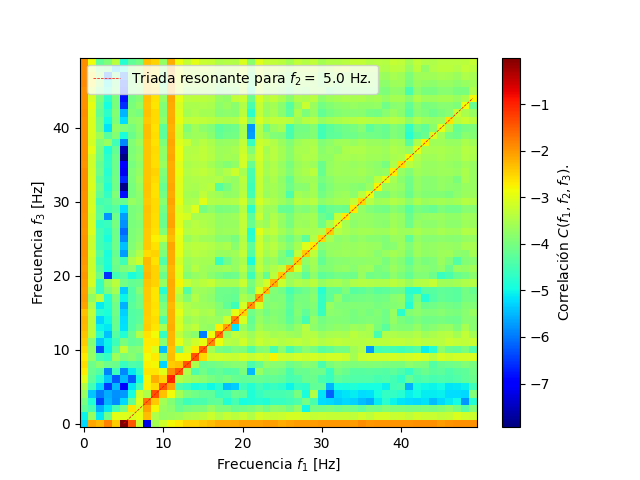
\includegraphics[width=0.89\textwidth]{Figures/01_09_2025/Correlación_3_ondas_ventana_1s.png}
							\captionsetup{width=0.8\textwidth}
							\subcaption{Tres ondas.} %  
							% \label{fig:}
						\end{subfigure}
			\end{minipage}\begin{minipage}[c]{0.49\textwidth}
				\begin{subfigure}{\textwidth}
							\centering
							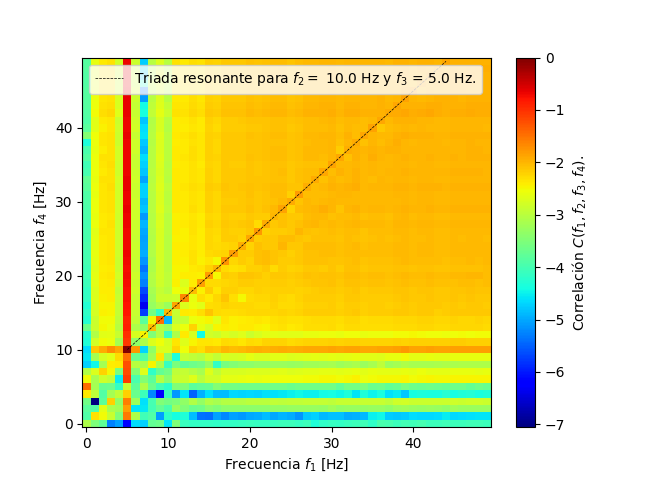
\includegraphics[width=0.89\textwidth]{Figures/01_09_2025/Correlación_4_ondas_ventana_1s.png}
							\captionsetup{width=0.8\textwidth}
							\subcaption{Cuatro ondas.} %  
							% \label{fig:}
						\end{subfigure}
			\end{minipage}
	\caption{Correlación de 3 y 4 ondas para la banda 0 - 6 Hz haciendo promedio en muchas ventanas temporales con overlap. } % a 
	\label{fig:waves_correlation_only_window_average}
\end{figure}

Primero calculé estas correlaciones fijando para el caso de tres ondas $f_2=10$ Hz y para la de cuatro ondas $f_2=10$ Hz y $f_3=5$ Hz. Los resultados son los que están a continuación.

Podemos notar que en los dos casos aparecen líneas de correlación máxima cuando se cumplen las condiciones resonantes: 

\begin{equation}
	f_1 = f_2 + f_3, \qquad f_1 + f_2 = f_3 + f_4  
\end{equation}

Ya que en esas condiciones la fase del producto de las $\eta(\omega)$ se anularía, considerando el signo de los conjugados para que esto pase. Para que aparezcan las líneas tengo que poner mucho overlap para tener la mayor cantidad de ventanas posibles en el promedio.

Si quiero aumentar la resolución de 1 Hz como está en los gráficos anteriores a más, por ejemplo a 0.1 Hz usando ventanas de 10 s, empiezan a aumentar réplicas de la línea, indicando resonancias de la forma $f_1=f_2+f_3+n\Delta f$. Esto pareciera ser sin embargo un artificio del análisis de los datos, tal vez por la no periodicidad de los datos en las ventanas. %  sin embargo, 


\begin{figure}[th!]
	\centering
	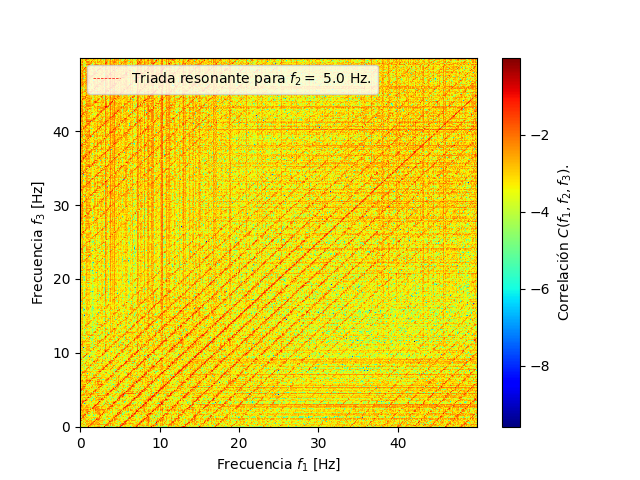
\includegraphics[width=0.49150587\linewidth]{Figures/01_09_2025/Correlación_3_ondas_ventana_10s}
	\caption{Correlación de tres ondas con $f_2=5$ Hz y ventanas de 10 segundos.}
	\label{fig:correlacion3ondasventana10s}
\end{figure}

Después de esto probé otras cosas, en un primer lugar aplicar a ventanas a cada ventana temporal, en este caso particular usé Hanning, para que sean periódicas las señales y evitar problemas por ese lado. Noté que esto me sacó las líneas verticales y horizontales en $C$. 

%  x
\begin{figure}[!ht]
	\begin{minipage}[c]{0.5\textwidth}
		\begin{subfigure}{\textwidth}
			\centering
			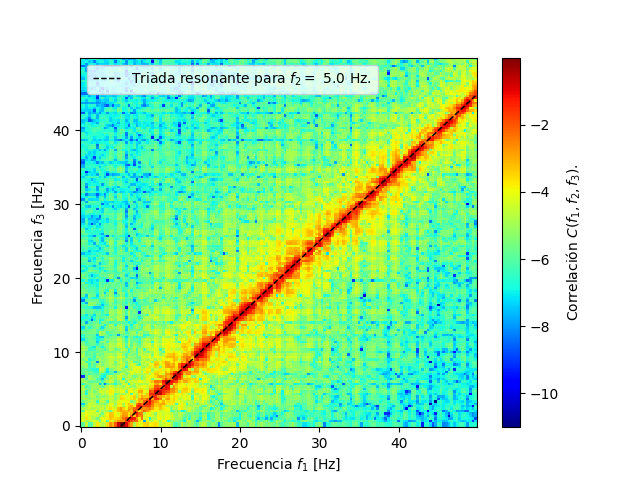
\includegraphics[width=0.98\textwidth]{Figures/01_09_2025/Correlación_3_ondas_ventana_3s_hanning_conditional.png}
			\captionsetup{width=0.8\textwidth}
			\subcaption{.}
			% \label{fig:}
		\end{subfigure}
	\end{minipage}\begin{minipage}[c]{0.49\textwidth}
		\begin{subfigure}{\textwidth}
			\centering
			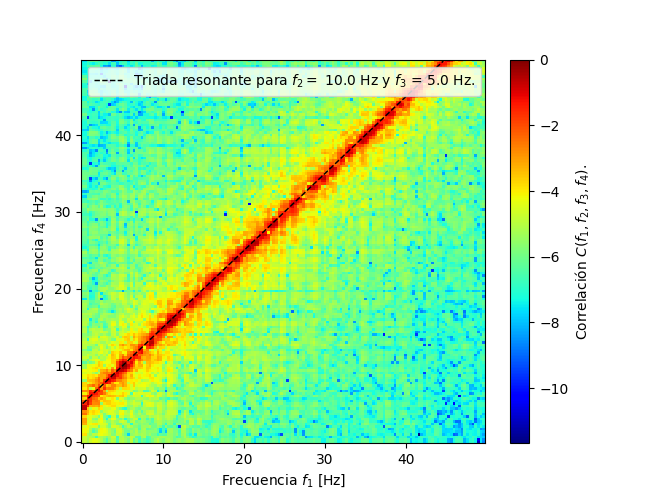
\includegraphics[width=0.98\textwidth]{Figures/01_09_2025/Correlación_4_ondas_ventana_3s_hanning_conditional.png} % a
			\captionsetup{width=0.8\textwidth}
			\subcaption{.}
			% \label{fig:}
		\end{subfigure}
	\end{minipage}
	\caption{Mismo que Figura \ref{fig:waves_correlation_only_window_average} con más resolución, pero aplicando una ventana Hann a cada ventana de datos (que saca las líneas verticales y horizontales) y conditional average (que saca las réplicas de las diagonales). }
	\label{fig:waves_correlation_hanning_plus_conditional_average}
\end{figure} 

Después, apliqué lo que definen en \cite{campagneIdentifyingFourWave2019} como promedio condicional. Esto consiste en utilizar solo ventanas donde se verifique la condición $|\partial_t\eta|<3.5v_{\text{rms}}$, con $v_{\text{rms}}=\sqrt{\langle(\partial_t)^2\rangle_t}$ de TODA la medición. Este criterio es ya que aquellas señales con velocidad a tantos sigmas de la media probablemente sean no Físicas, y más bien artificios de la técnica de medición. En mi caso esto saca los empalmes que quedan entre las ventanas de la aplicación del Lock-in, pero solo la mitad de las ventanas que venía usando cumplían el criterio, con lo cual tuve que aumentar mucho el overlap (a tipo $99.5-99.9$ \%). Cuanto más ventanas usase más de las réplicas diagonales sacaba, hasta llegar a lo de la Figura \ref{fig:waves_correlation_hanning_plus_conditional_average}.  % siguiente 


Por último calculé la correlación de 3 ondas no para un valor particular de $f_2$ sino para un barrido, pudiendo notar que la condición resonante se cumple en todas las frecuencias, formando el plano $f_1=f_2+f_3$. Estuve probando varias formas de visualizar este resultado, algunas más abajo. 

\begin{figure}[!ht]
	\begin{minipage}[c]{0.5\textwidth}
		\begin{subfigure}{\textwidth}
			\centering
			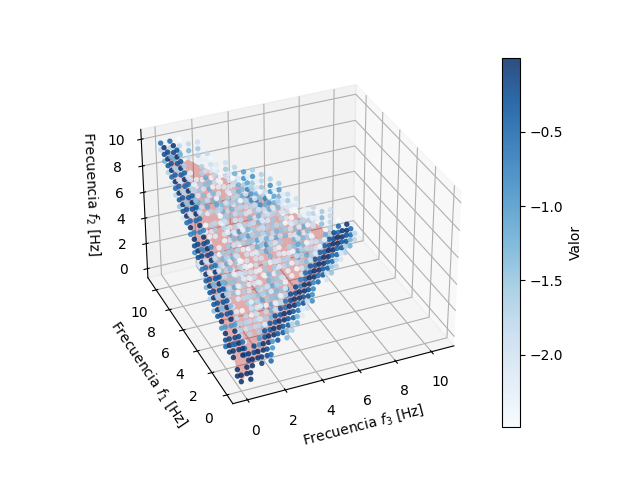
\includegraphics[width=0.98\textwidth]{Figures/01_09_2025/Correlación_3_ondas_ventana_volumen_completo_threshold.png}
			\captionsetup{width=0.8\textwidth}
			\subcaption{Threshold de los datos y scatter con plano $f_1=f_2+f_3$ superpuesto.}
			% \label{fig:}
		\end{subfigure}
	\end{minipage}\begin{minipage}[c]{0.49\textwidth}
		\begin{subfigure}{\textwidth}
			\centering
			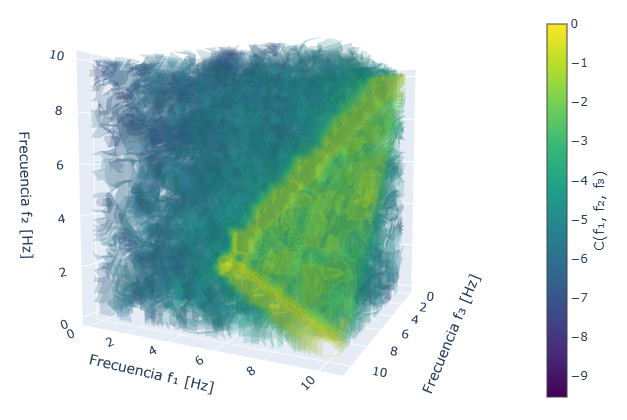
\includegraphics[width=0.98\textwidth]{Figures/01_09_2025/Correlación_3_ondas_ventana_volumen_completo_plotly.PNG}
			\captionsetup{width=0.8\textwidth} 
			\subcaption{Isovolumen con Plotly.}
			% \label{fig:}
		\end{subfigure}
	\end{minipage}
	
	\begin{minipage}[c]{0.49\textwidth}
		\begin{subfigure}{\textwidth}
			\centering
			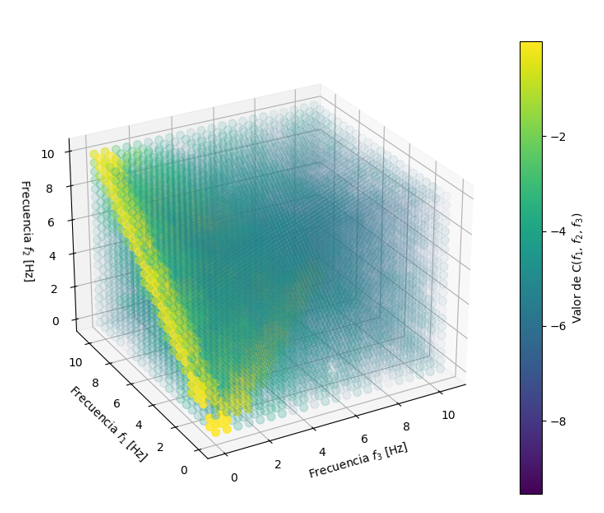
\includegraphics[width=0.98\textwidth]{Figures/01_09_2025/Correlación_3_ondas_ventana_3s_hanning_conditional_volumen_completo_v0.png}
			\captionsetup{width=0.8\textwidth}
			\subcaption{Canal A de RGBA como intensidad normalizada, con poca atenuación.}
			% \label{fig:} 
		\end{subfigure}
	\end{minipage}\begin{minipage}[c]{0.49\textwidth}	
		\begin{subfigure}{\textwidth}
			\centering
			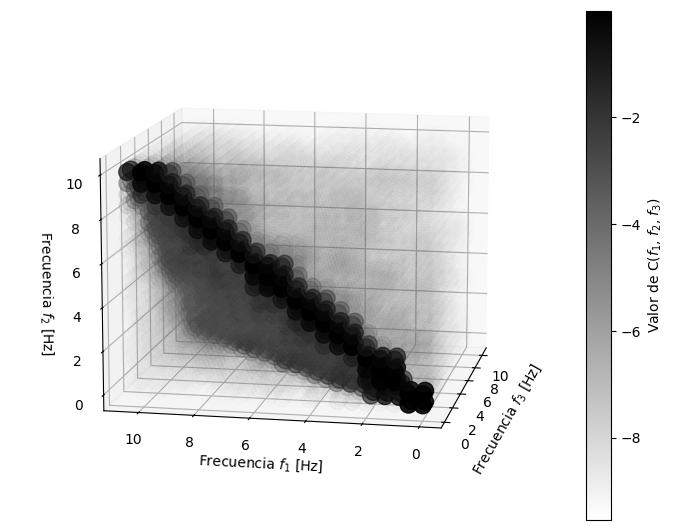
\includegraphics[width=0.98\textwidth]{Figures/01_09_2025/Correlación_3_ondas_ventana_3s_hanning_conditional_volumen_completo.png}
			\captionsetup{width=0.8\textwidth}
			\subcaption{Canal A de RGBA como intensidad normalizada, con más atenuación.}
			% \label{fig:}
		\end{subfigure}
	\end{minipage}  
	\caption{Correlación de tres ondas normalizada $C(f_1,f_2,f_3)$ en un cubo de 10 Hz x 10 Hz x 10 Hz, en escala logarítmica. Distintas visualizaciones. }
\label{fig:whole_volume_three_wave_correlation}
\end{figure}	
	
Para terminar podemos definir también la bicoherencia para tres ondas como: 

\begin{equation}
	B(\omega_2, \omega_3) = C(\omega_1=\omega_2+\omega_3, \omega_2, \omega_3) 
\end{equation}	

Aunque esta no dio muy parecida a lo reportado por \cite{aubourgNonlocalResonancesWeak2015}, donde se debería notar el $\omega_3^{\text{mín}}$ a partir del cual es posible que se cumpla la condición resonante. Sí se nota la simetría respecto a la línea $f_2=f_3$. 
	
\begin{figure}[!ht]
	\begin{minipage}[c]{0.5\textwidth}
		\begin{subfigure}{\textwidth}
			\centering
			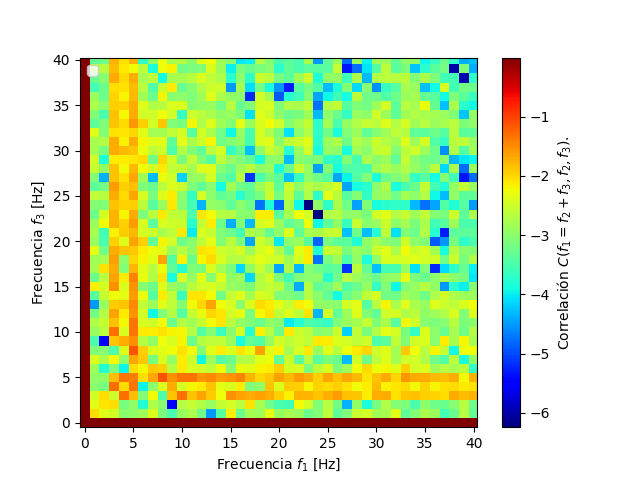
\includegraphics[width=0.98\textwidth]{Figures/01_09_2025/Bicoherencia_1s_5per_5cond.png}
			\captionsetup{width=0.8\textwidth}
			\subcaption{Ventana 1 s, overlap de 5 \%, conditional average, banda de 0 - 6 Hz, amplitud 50 \%.}
			% \label{fig:}
		\end{subfigure}
	\end{minipage}\begin{minipage}[c]{0.49\textwidth}
		\begin{subfigure}{\textwidth}
			\centering
			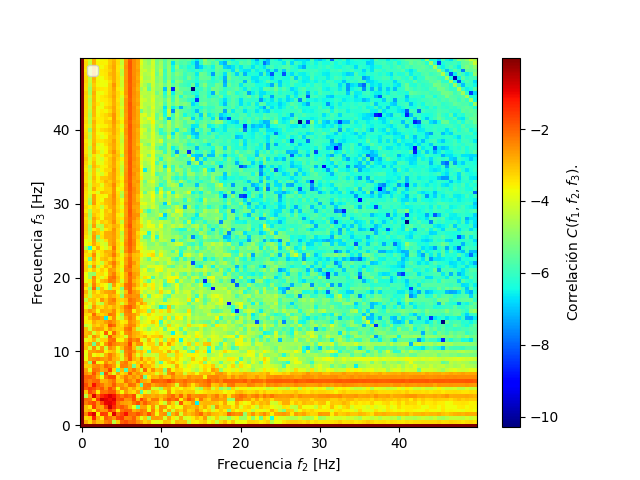
\includegraphics[width=0.98\textwidth]{Figures/01_09_2025/Bicoherencia_2s_95per_cond_amp50.png}
			\captionsetup{width=0.8\textwidth}
			\subcaption{Ventana 2 s, overlap 95 \%, conditional average, banda de 0 - 4 Hz con amplitud 50 \%.}
			% \label{fig:}
		\end{subfigure}
	\end{minipage}
	\caption{Bicoherencia normalizada $B(f_2, f_3)$ en escala logarítmica.}
	\label{fig:bicoherence_various}
\end{figure} 

También se debería notar en los gráficos de la correlación de 3 y 4 ondas que la línea arranca a partir de un $\omega^{\text{mín}}$, pero acá abarca todo el rango de frecuencias, tal vez ya que el forzado en la banda de 0 - 6 Hz ya se iba del débilmente no lineal y empezaban a aparecen Bound Waves que permitían otras interacciones resonantes por fuera de las que permitiría la relación de dispersión clásica. 



% TRES SUBFIGURAS HORIZONTALES.  
% 
%\begin{figure}[!ht]
%	\begin{minipage}[c]{0.325\textwidth}
%		\begin{subfigure}{\textwidth}
%			\centering
%			\includegraphics[width=0.8\textwidth]{}
%			\captionsetup{width=0.8\textwidth}
%			\subcaption{.}
%			\label{fig:}
%		\end{subfigure}
%	\end{minipage}\begin{minipage}[c]{0.3249\textwidth}
%		\begin{subfigure}{\textwidth}
%			\centering
%			\includegraphics[width=0.8\textwidth]{}
%			\captionsetup{width=0.8\textwidth}
%			\subcaption{.}
%			\label{fig:}
%		\end{subfigure}
%	\end{minipage}\begin{minipage}[c]{0.3249\textwidth}
%		\begin{subfigure}{\textwidth}
%			\centering
%			\includegraphics[width=0.8\textwidth]{}
%			\captionsetup{width=0.8\textwidth}
%			\subcaption{.}
%			\label{fig:}
%		\end{subfigure}
%	\end{minipage}
%	\caption{}
%	\label{fig:}
%\end{figure}
%
% DOS SUBFIGURAS HORIZONTALES.
% 
%\begin{figure}[!ht]
%	\begin{minipage}[c]{0.5\textwidth}
%			\begin{subfigure}{\textwidth}
%					\centering
%					\includegraphics[width=0.8\textwidth]{}
%					\captionsetup{width=0.8\textwidth}
%					\subcaption{.}
%					\label{fig:}
%				\end{subfigure}
%		\end{minipage}\begin{minipage}[c]{0.49\textwidth}
%			\begin{subfigure}{\textwidth}
%					\centering
%					\includegraphics[width=0.8\textwidth]{}
%					\captionsetup{width=0.8\textwidth}
%					\subcaption{.}
%					\label{fig:}
%				\end{subfigure}
%		\end{minipage}
%	\caption{}
%	\label{fig:}
%\end{figure}


 